\title{LEZIONE 19 21/05/20}
\textbf{link} \href{https://web.microsoftstream.com/video/9329ad3d-c8a8-48ab-b415-668ff6193e36?list=user&userId=cfe0965d-9a7c-40e2-be6e-f078296a1914}{clicca qui}
\section{Patter pure HTML vs RIA}
Architettura THIN:
\begin{center}
    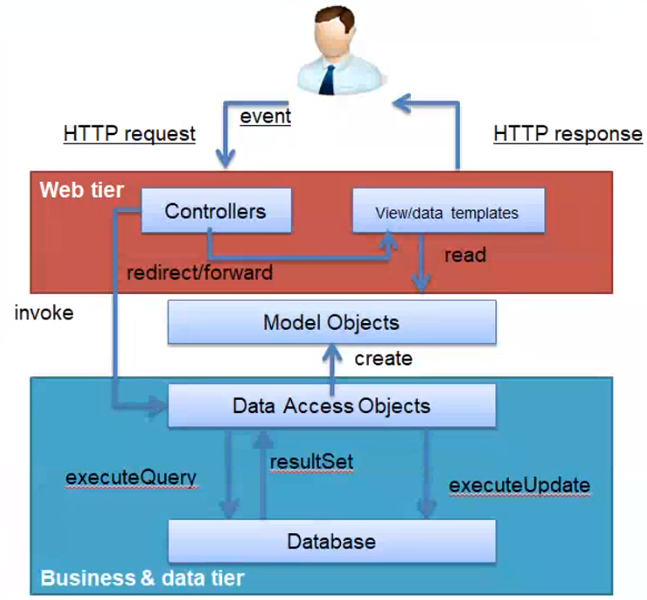
\includegraphics[height=4cm]{../lezione19/img1.PNG}
\end{center}
Architettura FAT:
\begin{center}
    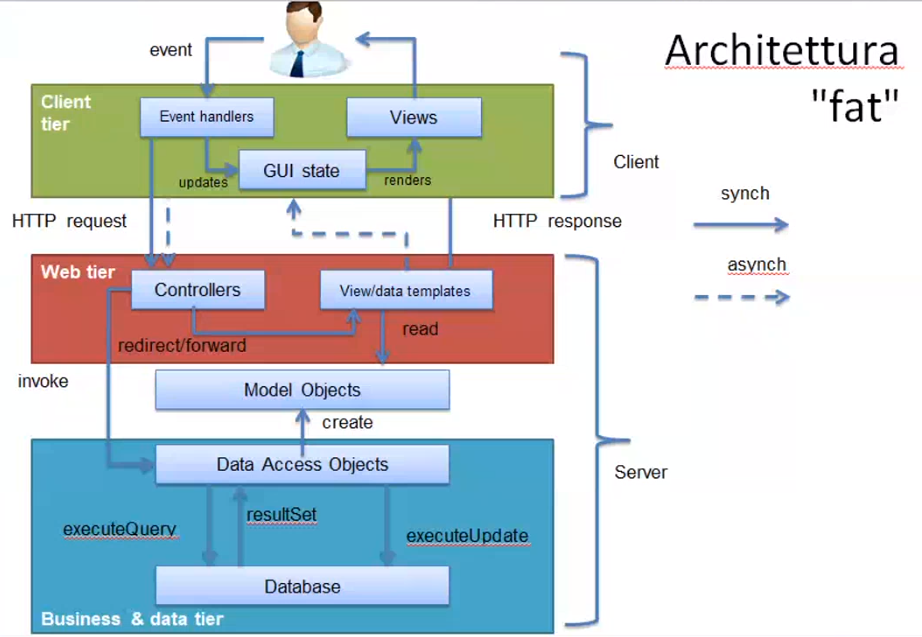
\includegraphics[height=5cm]{../lezione19/img2.PNG}
\end{center} 
\ \newline
Iniziamo osservando le differenze negli eventi.\newline
Pure HTML:
\begin{itemize}
    \item gli eventi sono richieste HTTP;
    \item gli eventi provengono dal client;
    \item gli eventi son ocreati dal browser che gestisce per default gli elementi ancora e i buttoni di submit;
    \item gli eventi sono ricevuti dal web server che li inoltra al servlet container (tomcat).
\end{itemize}
RIA:
\begin{itemize}
    \item gli eventi sono eventi di DOM e HTMLAPI;
    \item gli eventi provengono dal browser (oggetto window) o dal server (response HTTP);
    \item gli eventi sono prodotti dall'interazione dell'utente o dall'interfaccia di rete (oggetto XMLHttpRequest);
    \item gli eventi sono dal browser e notificati al gestore tramite l'oggetto contenitore window.
\end{itemize}